\section{Experiment and Evaluation}
\subsection{Setup and Metrics}


\subsection{Stress Buffering}{Stress-buffering Pattern of scheduled positive events}
%KTS
%five stressors
%Measures
%pre/post

Basically, we focused on four scheduled positive events:
\emph{practical activity}, \emph{holiday}, \emph{new year party} and \emph{sports meeting}.
For each of the four scheduled positive events,
we quantified the stress-buffering effect based on corresponding SI and U-SI interval sets of the 124 students.

\begin{figure*}
\centering
\includegraphics[width=0.9\linewidth]{figs/BOX3.eps}%figs/correlation2.eps
\caption{Stress-buffering pattern of positive events. Figure a) shows correlation of each microblog measure,
and figure b) shows stress-buffering effect on five dimensions of stress. 'KTS' means KNN-based correlation method.}
\label{fig:correlation}
\end{figure*}

\begin{table}[H]
\begin{center}
\caption{\small{Quantify the impact of scheduled positive school events using KTS (the KNN-based two sample method adopted in this research) and baseline method.}}
\label{tab:schedule}
\resizebox{0.45\textwidth}{13mm}{
\small{
\begin{tabular}{lccccc}
\toprule
&	\emph{practical}	&	         	&	\emph{new year}	&	\emph{sports}	&	\emph{}	\\
&	\emph{activity}	&	\emph{holiday}	&	\emph{party}	&	\emph{meeting}	&	\emph{all}	\\
\midrule
size of U-SI	&	219 	&	339 	&	235 	&	226 	&	1,019 	\\
Pearson         &55.65\%	&	70.97\%	&	56.45\%	&	54.84\%	&	65.32\% \\
KTS             &54.52\%	&	78.39\%	&	63.39\%	&	58.74\%	&	69.52\% \\
\bottomrule
\end{tabular}
}
}
\end{center}
\end{table}

Table \ref{tab:schedule} shows the experimental results,
where 54.52\%, 78.39\%, 63.39\%, 58.74\% significant stress-buffering effect were detected for the four specific scheduled positive events,
with the total ratio to 69.52\% ($\alpha$ =1.96 for p=0.025).
We adopted the commonly used Pearson correlation algorithm to compare with the two sample statistical method in this study.
The Euclidean metric was used to calculate the distance between two $n$ dimension points $X$ and $Y$.
Experimental results show that our KNN-based two sample method (denoted as KTS) outperformed the baseline method
with the best improvement in \emph{new year party} to 10.94\%,
and total improvement to 6.00\%.


\begin{table*}
\begin{center}
\caption{\small{Monotonous stress intensity changes in U-SI and SI intervals compared with adjacent intervals.}}
%\resizebox{\textwidth}{15mm}{
\small{
\begin{tabular}{l cccccc cccccc} \\\hline\hline
\multirow{2}{1cm}{}
&\multicolumn{2}{c}{school life}
&\multicolumn{2}{c}{romantic}
&\multicolumn{2}{c}{peer relationship}
&\multicolumn{2}{c}{self-cognition}
&\multicolumn{2}{c}{family life}
&\multicolumn{2}{c}{all types}\\
&U-SI	    &	SI	        &U-SI	    &SI	        &U-SI	   &SI	
&U-SI	    &	SI	        &	U-SI	&SI	        &U-SI	   &SI\\  \hline
\# interval         &   365	        &	514	        &	536	        &	587	        &128	    &	391	        &	564	           &	609	            &	321	        &	481	        &	1,914	    &2,582	 \\
front $\rightarrow$ I &	72.60\% &	78.79\% &	69.03\% 	&77.51\%   &74.22\%    &81.59\%    &70.04\%    &77.67\%  &67.91\%     &77.96\%    &70.17\%    &78.51\% \\
I $\rightarrow$ rear  &	75.89\% &	78.40\% &	74.63\% 	&79.05\%   &78.13\%    &82.61\%    &75.00\%    &79.15\%   &74.14\%    &79.42\%    &75.13\%    & 79.55\%\\ \hline \hline
\end{tabular}}%}}
\label{tab:fontrear}
\end{center}
\end{table*}

The correlation of positive events a) in each group of microblog measure
and b) towards five dimensions of stress
were shown in box-plots \ref{fig:correlation}.
The stress-buffering pattern of positive events
was closely correlated with posting behavior (ratio = 80.65\%, n=100, SD=1.96),
stress change mode (ratio = 67.74\%, n=84, SD=2.04) and microblog linguistic expressions (ratio = 74.19\%, n=92, SD=2.07).
Positive events conducted most intensive stress-buffering impact on 'family life' (ratio = 83.87\%, n=104, SD=2.72),
followed by 'peer relationships' (ratio = 71.77\%, n=89, SD=4.04) and 'school life' (ratio = 67.74\%, n=84, SD=2.71) dimensions.
The correlation values in 'peer relation'
exhibited the highest 75th percentile while the lowest 25th percentile,
showing a relatively random and unstable stress-buffering effect on this dimension.
Comparing the hypothesis test results on scheduled positive events (ratio = 69.52\%)
and automatically extracted positive events (ratio = 74.21\%),
the result indicated the feasibility of automatically extracting positive events from microblogs.
%%����Ϊcorrelation

\subsection{Stress Prediction}
